\documentclass[11pt]{beamer}
\usetheme{Dresden}
%\usecolortheme{beaver}
\usepackage[utf8]{inputenc}
\usepackage{amsmath}
\usepackage{amsfonts}
\usepackage{amssymb}
\usepackage{graphicx}
\usepackage{listings}
\usepackage{verbatim}
\author{NCC Moore}
\title{Topic 7 - Benchmarking, Profiling and Advanced Bash Commands}
%\setbeamercovered{transparent} 
%\setbeamertemplate{navigation symbols}{} 
%\logo{} 
\institute{McMaster University} 
\date{Summer 2021} 
\subject{COMPSCI 1XC3 - Computer Science Practice and Experience: Development Basics} 
\stepcounter{section}

\definecolor{mGreen}{rgb}{0,0.6,0}
\definecolor{mGray}{rgb}{0.5,0.5,0.5}
\definecolor{mPurple}{rgb}{0.58,0,0.05}
\definecolor{mGreen2}{rgb}{0.05,0.65,0.05}
\definecolor{mGray2}{rgb}{0.55,0.55,0.55}
\definecolor{mPurple2}{rgb}{0.63,0.05,0.05}
\definecolor{backgroundColour}{rgb}{0.95,0.95,0.92}
\definecolor{backgroundColour2}{rgb}{0.95,0.92,0.95}

\lstdefinestyle{C}{
    backgroundcolor=\color{backgroundColour},   
    commentstyle=\color{mGreen},
    keywordstyle=\color{blue},
    numberstyle=\tiny\color{mGray},
    stringstyle=\color{mPurple},    
    basicstyle=\footnotesize,
    breakatwhitespace=false,         
    breaklines=true,                 
    captionpos=b,                    
    keepspaces=true,                 
    numbers=left,                    
    numbersep=5pt,                  
    showspaces=false,                
    showstringspaces=false,
    showtabs=false,                  
    tabsize=2,
    language=C
}

\definecolor{t_comment}{rgb}{0.2,1,0.2}
\definecolor{t_mGray}{rgb}{0.5,0.5,0.5}
\definecolor{t_mPurple}{rgb}{0.58,0,0.05}
\definecolor{t_blue}{rgb}{0.4,0.6,0.8}
\definecolor{t_mGreen2}{rgb}{0.05,0.65,0.05}
\definecolor{t_mGray2}{rgb}{0.75,0.75,0.75}
\definecolor{t_mPurple2}{rgb}{0.63,0.05,0.05}
\definecolor{t_bg}{rgb}{0.15,0.15,0.18}

\lstdefinestyle{terminal}{
    backgroundcolor=\color{t_bg},   
    commentstyle=\color{t_comment},
    keywordstyle=\color{t_blue},
    numberstyle=\tiny\color{t_mGray},
    stringstyle=\color{t_mGray2}, 
    basicstyle=\footnotesize\color{t_mGray2},
    breakatwhitespace=false,         
    breaklines=true,                 
    captionpos=b,                    
    keepspaces=true,                 
    numbers=none,                    
    numbersep=5pt,                  
    showspaces=false,                
    showstringspaces=false,
    showtabs=false,                  
    tabsize=2,
    language=C
}

\definecolor{eggplant}{rgb}{0.5, 0.25, 0.5} % UBC Blue (primary)

\usecolortheme[named=eggplant]{structure}

\begin{document}

\begin{frame}
\center
COMPSCI 1XC3 - Computer Science Practice and Experience:
Development Basics
\titlepage
% Toggle for C chapters
% Adapted from C: How to Program 8th ed., Deitel \& Deitel
\end{frame}

\begin{frame}
\tableofcontents
\end{frame}

\section[htop]{Viewing Processes Using \texttt{htop}}
\begin{frame}{Viewing Processes Using \texttt{htop}}
\center

\includegraphics[scale=0.25]{htop.jpg} \\
``It's like crtl+alt+del for Linux!''  \\
``It's crtl+shift+esc now.'' \\
``... of course it is.''
\end{frame}

\begin{frame}{\texttt{htop} O' the Morning to Ya!}
Modern operating systems manage hundreds, even thousands of concurrently executing programs.
\begin{itemize}
\item These are known as \textbf{processes}.  Each has a unique \textbf{process identification number}, or \emph{PID}.
\item One program may spawn many separate processes, known as \textbf{threads}.
\item Process management and scheduling is the subject of such courses as:
\begin{itemize}
\item COMPSCI 3SD3 - Concurrent Systems
\item COMPSCI 4DC3 - Distributed Computing
\end{itemize}
\end{itemize}
We can view information about our computers' currently open processes by calling \texttt{htop}.
\end{frame}

\begin{frame}{\texttt{htop} in Action}
\center
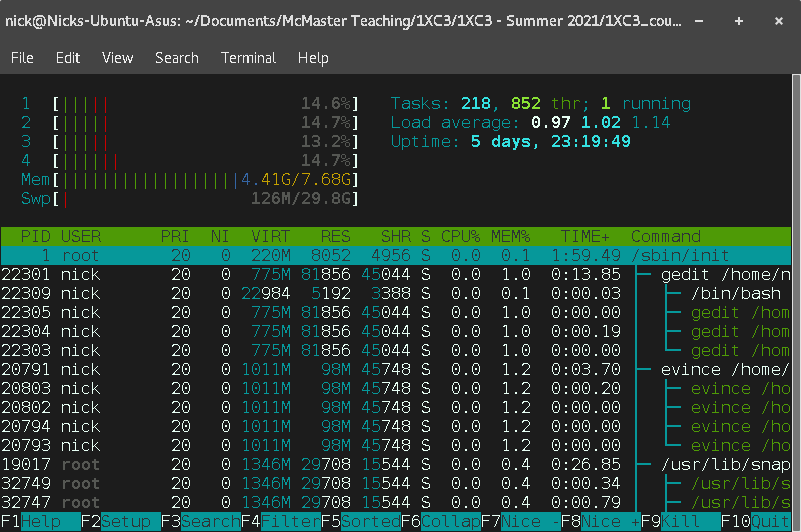
\includegraphics[scale=0.3]{htop2.png}
\end{frame}

\begin{frame}{Useful Things to Know!}
Among the information displayed is:
\begin{itemize}
\item Percent utilization of each CPU core in your computer.
\item Memory usage out of total available memory.
\item Swap space usage.
\item The number of processes and threads currently running.
\item How long it's been since you turned off your computer.  
\end{itemize}
For each individual processes, you can easily see...
\begin{itemize}
\item Memory and CPU usage. 
\item Origin within the file system
\item Which user is running it
\end{itemize}
You can use \texttt{htop} to \emph{terminate} processes!  Hasta la vista, baby!  
\end{frame}

\section[time]{Benchmarking using \texttt{time}}
\begin{frame}{Benchmarking!}
\textbf{Benchmarking} is the practice of measuring a product's features or performance, and comparing the results to other products of a similar nature.
\begin{itemize}
\item The term derives from the $19^{th}$ century.  A benchmark was a channel cut into stone to mount measuring equipment.
\item In Hardware, benchmarking involves executing batch operations that push the hardware to its limits.
\item In Software, we are typically interested in \emph{time} and \emph{memory} performance.  
\end{itemize}
With \texttt{htop}, we can see these parameters for active processes, but what about processes that take a fraction of a second?  We need a stopwatch program! 
\end{frame}

\begin{frame}[fragile=singleslide]{The Nick of \texttt{time}}
\begin{lstlisting}[style=terminal]
$ time <the command you wish to time>
\end{lstlisting}
After executing this command, and once your program terminates, you'll get a report such as the following:
\begin{lstlisting}[style=terminal]
real	2m4.352s
user	0m58.341s
sys	1m49.005s
\end{lstlisting}
\begin{itemize}
\item \textbf{real} - the difference between the time the process started and the time it stopped.  This includes time the process was waiting for input or other processes.
\item \textbf{user} - time spent in user-mode code (your code plus libraries).  The amount of time the CPU used executing the process.  
\item \textbf{sys} - time spent in system-mode code (system calls and kernel stuff). 
\end{itemize}
\end{frame}

\begin{frame}[fragile=singleslide]{Aaaaand... That's \texttt{time}!}
You can also use the GNU version of \texttt{time} to track memory usage! 
\begin{lstlisting}[style=terminal]
$ /usr/bin/time -v <the command you wish to time>
\end{lstlisting}
Bash has its own version of \texttt{time} which it defaults to, so we have to specify the full path of the GNU version.  
\begin{itemize}
\item The \texttt{-v} flag specifies ``verbose'' mode. This produces a lot of statistics on our command's execution:
\begin{itemize}
\item Maximum resident set size - The maximum amount of physical memory your process was allocated by the operating system.  
\item Exit status - the integer that your command returned.  Non-zero statuses indicate ``abnormal exit''
\end{itemize}
\item It also tracks things like filesystem interactions and network usage.  
\end{itemize}

\center
\emph{While \texttt{time} gives you a quick, rough idea of how many resources your program is using, you'll often need more detail than this.}
\end{frame}

\section[gprof]{Profiling using \texttt{gprof}}
\begin{frame}{Optimization!}
\center
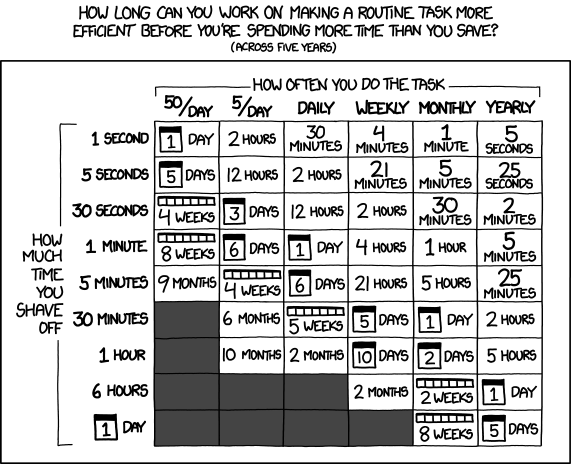
\includegraphics[scale=0.4]{optimizing.png}
\end{frame}

\begin{frame}{Introducing... \texttt{gprof}, the GNU profiling utility!}
\texttt{htop} gives us a good idea of our system load, and \texttt{time} is good for fast estimations of runtime and memory usage, but these programs do not tell us anything about our program's \emph{structure}!
\begin{itemize}
\item \textbf{Profiling} lets us break down our program's structure, and view statistics about the use of individual functions.  
\item This information can be used to help us optimize our programs.
\begin{itemize}
\item Profiling doesn't tell you \emph{how} to optimize.
\item Profiling does tell you \emph{where} to optimize.
\end{itemize}
\end{itemize}
\end{frame}

\begin{frame}{Autobots, Optimize!}
Before we profile our code, let's learn how to use \texttt{gcc}'s automatic optimization flags! 
\begin{itemize}
\item \texttt{-O} $\rightarrow$ Standard Optimization.
\item \texttt{-O2} $\rightarrow$ Level 2 Optimization.
\item \texttt{-O3} $\rightarrow$ Level 3 Optimization.
\item \texttt{-Os} $\rightarrow$ Size Optimization.
\item \texttt{-Ofast} $\rightarrow$ Speed Optimization. 
\item \texttt{-Og} $\rightarrow$ Debuggability Optimization.
\end{itemize}
Notes about Optimization:
\begin{itemize}
\item These options will actually re-arrange your source code.
\item You should be done debugging before using these.
\item Optimization takes time!  Especially for larger programs.
\end{itemize}
\end{frame}

\begin{frame}[fragile=singleslide]{Compiling for \texttt{gprof}}
\texttt{gprof} requires code to be inserted into your source files by \texttt{gcc}, so it can keep track of things.  
\begin{enumerate}
\item Compile your program using the -pg option
\begin{lstlisting}[style=terminal]
$ gcc -pg example.c -o example
\end{lstlisting}
\item Execute your program as normal to collect the statistics in the file \texttt{gmon.out}
\begin{lstlisting}[style=terminal]
$ ./example
\end{lstlisting}
\item Run \texttt{gprof} in the following manner:
\begin{lstlisting}[style=terminal]
$ gprof example > profilerResults.out
\end{lstlisting}
\item View the generated file, which has lots of tasty information! 
\end{enumerate}
\end{frame}


\begin{frame}[fragile = singleslide]{A Flat Profile}
\footnotesize
\begin{verbatim}
Each sample counts as 0.01 seconds.
  %   cumulative   self              self     total
 time   seconds   seconds    calls  ms/call  ms/call  name
 33.34      0.02     0.02     7208     0.00     0.00  open
 16.67      0.03     0.01      244     0.04     0.12  offtime
 16.67      0.04     0.01        8     1.25     1.25  memccpy
 16.67      0.05     0.01        7     1.43     1.43  write
 16.67      0.06     0.01                             mcount
  0.00      0.06     0.00      236     0.00     0.00  tzset
  0.00      0.06     0.00      192     0.00     0.00  tolower
  0.00      0.06     0.00       47     0.00     0.00  strlen
  0.00      0.06     0.00       45     0.00     0.00  strchr
  0.00      0.06     0.00        1     0.00    50.00  main
  0.00      0.06     0.00        1     0.00     0.00  memcpy
[...]
\end{verbatim}
\end{frame}

\begin{frame}{Interpretting the Flat Profile}
The flat profile provides the following information for every function your program uses (yes, even libraries).
\begin{itemize}
\item \textbf{\% time} $\rightarrow$ The percentage of total runtime the programe spent on each function.
\item \textbf{cumulative seconds} $\rightarrow$ The number of seconds spent in this function plus all entries above it in the table  
\item \textbf{self seconds} $\rightarrow$ Number of seconds spent in this function alone.
\item \textbf{calls} $\rightarrow$ Total number of times this function was called.
\item \textbf{self ms/call} $\rightarrow$ Average time spent in this function per call.
\item \textbf{total ms/call} $\rightarrow$ Averge time spent in this function \emph{and descendents} per call.
\item \textbf{name} $\rightarrow$ The name of the function
\end{itemize}
\end{frame}


\begin{frame}[fragile=singleslide]{A Call Graph}
\center
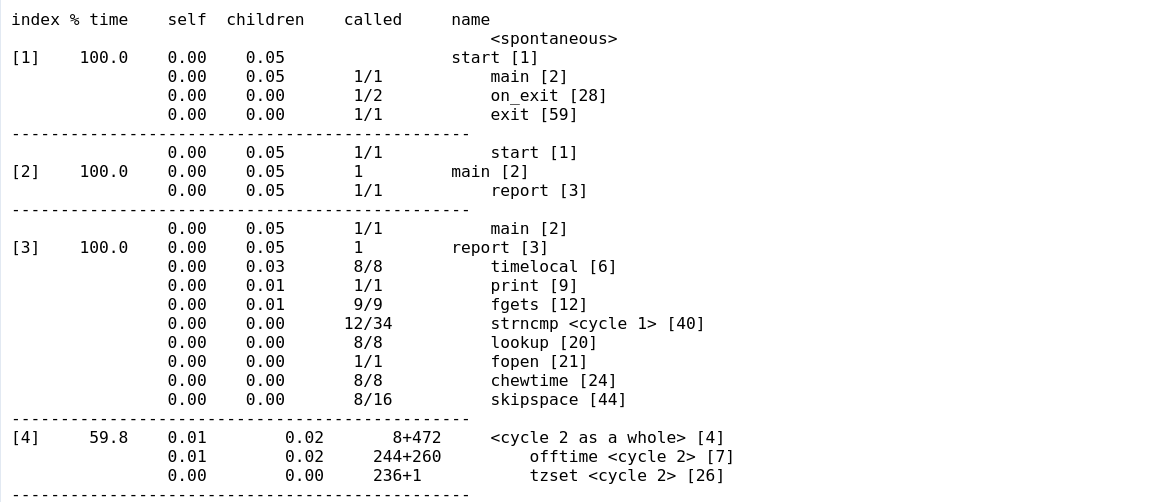
\includegraphics[scale=0.28]{CallGraph1.png}
\flushleft
The call graph gives you an idea of how many times each function is called by every other function in your program.  
\end{frame}


\begin{frame}{Interpretting the Call Graph}
\center
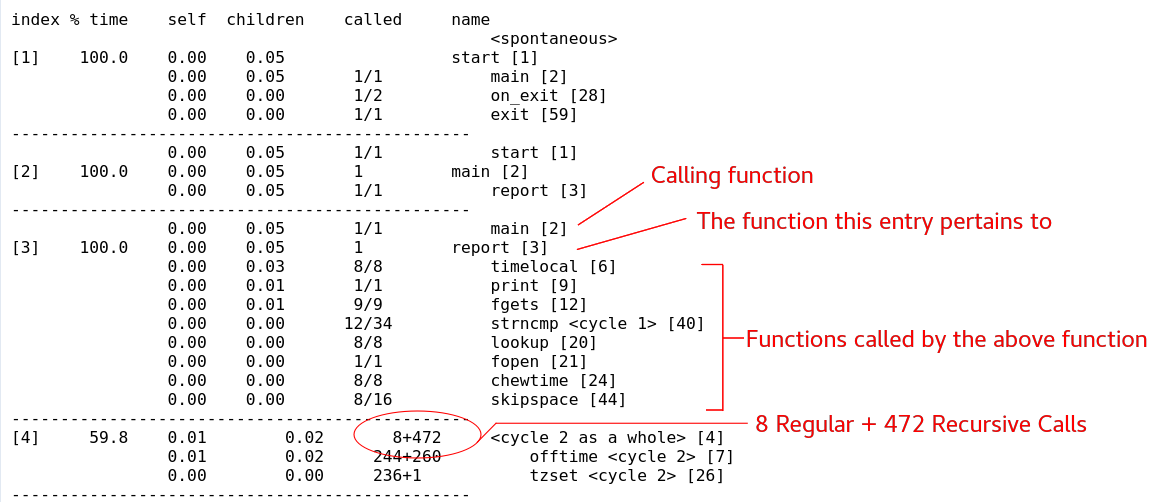
\includegraphics[scale=0.28]{CallGraph2.png}
\end{frame}

\begin{frame}{Call Graph Diagram}
Taking the above information and arranging it into a call graph diagram yields the following:

\center
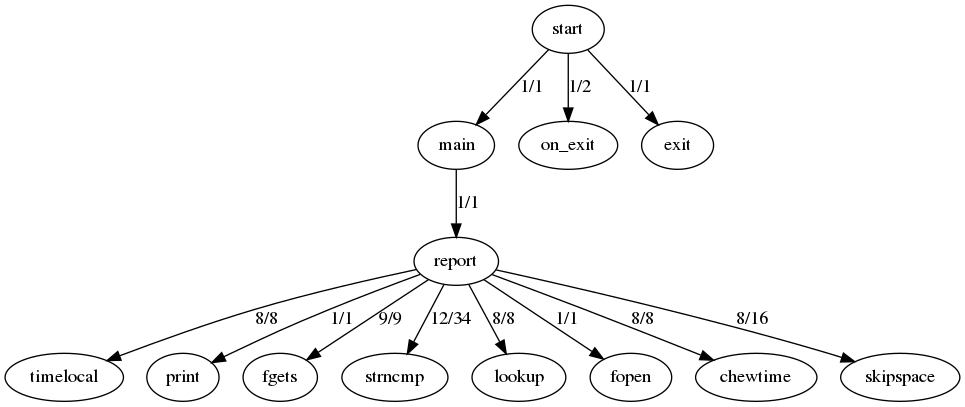
\includegraphics[scale=0.33]{graphs/callgraph.png}
\end{frame}

\section[gcov]{Source Code Annotation using \texttt{gcov}}
\begin{frame}{Source Code Annotation using \texttt{gcov}}
So, now we know how to profile code at the level of \emph{functions}, but \emph{we can go deeper!}
\begin{itemize}
\item \texttt{gcov} will annotate your source code itself with: 
\begin{itemize}
\item How often each line of code is executed
\item What lines of code are actually executed
\item How much computer time each section of code requires.
\end{itemize}
\item \texttt{gcov} is fantastic to use in combination with a testing, because it will tell you whether your tests have full coverage of the source code!
\end{itemize}
In order for the results to be meaningful, however, we can't use compiler optimizations, since they change the source code!
\end{frame}

\begin{frame}[fragile=singleslide]{Using \texttt{gcov}}
To use \texttt{gcov}, we need once again to perform a special compilation:
\begin{lstlisting}[style=terminal]
$ gcc -fprofile-arcs -ftest-coverage example.c
\end{lstlisting}
Take the resulting executable file and execute it.  This will produce a \texttt{*.gcda} file, which contains the profiling data. Then invoke:
\begin{lstlisting}[style=terminal]
$ gcov example.c
\end{lstlisting}
The profiling results will be stored in \texttt{example.c.gcov}.
\end{frame}

\begin{frame}[fragile=singleslide]{Interpretting the Output}
\footnotesize
\begin{lstlisting}[style=C]
[...]
// <Execution count> : <Line number> : <Source Code>
        5:  123:	int xcheck = x1;
        5:  124:	int ycheck = y1;
        5:  125:	int piecesInWay = 0;
        5:  126:	if (x1 > 7 || x1 < 0) {
        1:  127:		return false;
        4:  128:	} else if (y1 > 7 || y1 < 0) {
    #####:  129:		return false;
        4:  130:	} else if (x2 > 7 || x2 < 0) {
    #####:  131:		return false;
        4:  132:	} else if (y2 > 7 || y2 < 0) {
    #####:  133:		return false;
        -:  134:	}
// "#####" indicates the line was not executed, i.e., not "covered"
[...]
\end{lstlisting}

\end{frame}

\section[Permissions]{Random Topic: File Permissions in Unix}
\begin{frame}{Unix File Permissions}
\center
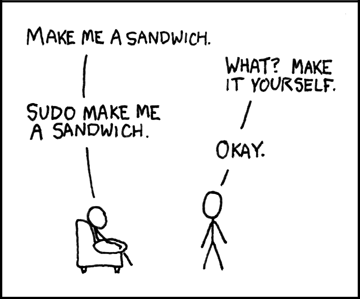
\includegraphics[scale=0.4]{sandwich.png} \\
``UNIX is basically a simple operating system, but you have to be a genius to understand the simplicity.''  \\ -- Dennis Ritchie
\end{frame}

\begin{frame}{Unix File Permissions}
Within the Unix file system, 10 bits are allocated per file to record file permissions, and are visible when using \texttt{ls -l}
\vspace{-1em}
\begin{columns}
\begin{column}{0.6\textwidth}
\center
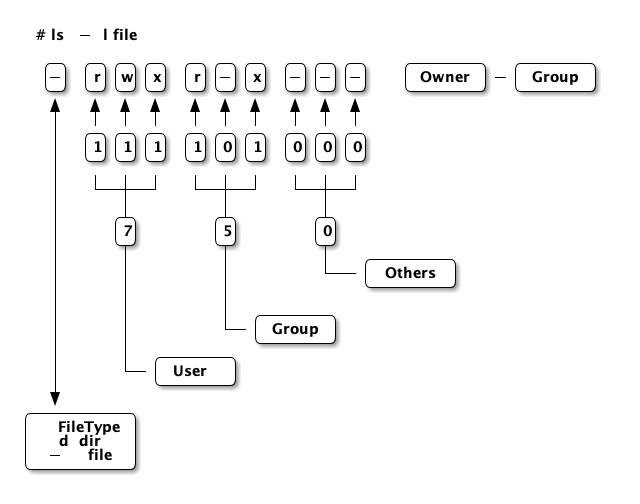
\includegraphics[scale=0.3]{permissions.png}
\end{column}
\begin{column}{0.4\textwidth}
Unix-like systems specify user permissions by:
\begin{itemize}
\item \textbf{User}
\item \textbf{Group}
\item \textbf{Others}
\end{itemize}
Specifying if a file is :
\begin{itemize}
\item \textbf{Readable}
\item \textbf{Writeable}
\item \textbf{Executable}
\end{itemize}
\end{column}
\end{columns}
\end{frame}

\begin{frame}{Filetype, User, Group and Others}
\begin{itemize}
\item \textbf{File Type} only specifies whether an item is a file or a directory.
\item \textbf{User} $\rightarrow$ Each file has an owner, these bit specify the permissions for the owner (this will be you most of the time).
\item \textbf{Group} $\rightarrow$ Users may be collected into groups for ease of management. 
\begin{itemize}
\item Group permissions apply to the group you are a member of (if any).
\item Think of the difference between \emph{student} and \emph{faculty} access to something like Avenue or Mosaic.  
\end{itemize}
item \textbf{Others} $\rightarrow$ Permissions for everyone not in the first two categories.  
\end{itemize}
\end{frame}

\begin{frame}[fragile=singleslide]{It's a bird! It's a Plane! It's Superuser!}
If you're trying to do something in Unix/Linux, and you get \texttt{ Permission denied}, that means you don't have the correct level of privilege for the operation you are trying to perform.
	\begin{itemize}
	\item There is only one way around this: invoking SUPERUSER!
	\end{itemize}
\begin{lstlisting}[style=terminal]
$ sudo <command you weren't able to execute>
\end{lstlisting}
	\begin{itemize}
	\item In Linux, the superuser account (called ``root'') is omnipotent, with unrestricted access to:
		\begin{itemize}
		\item commands, files, directories, and resources.
		\item This also means the ability to install programs for all users, change system settings, and \emph{compile that kernel!}
		\end{itemize}
	\item granting and revoking permissions for other users.
	\end{itemize}
The main difference between having a linux system or virtual machine and logging into the pascal server is that you don't have sudo priveleges on pascal for obvious reasons! 
\end{frame}



\begin{frame}[fragile=singleslide]{The Group Scoop}
By default, each user is already in a group containing just itself.
\begin{itemize}
\item This group's name is the user's name.
\item You can create a group (assuming you have the authority to do so) as follows:
\end{itemize}
\begin{lstlisting}[style=terminal]
$ groupadd <group name>
\end{lstlisting}
You can add a user to a group with...
\begin{lstlisting}[style=terminal]
$ useradd -g <user name> <group name>
\end{lstlisting}
\end{frame}

\begin{frame}[fragile=singleslide]{Modifying File Permissions via \texttt{chmod}}
\begin{lstlisting}[style=terminal]
$ chmod u+x <file name>
    # add executable permissions to user
$ chmod o+rw <file name>
    # add read and write permission to others
$ chmod -w <file name>
    # remove write permissions from everyone
\end{lstlisting}
In general, it's 
\begin{lstlisting}[style=terminal]
$ chmod <person(s)><grant / revoke><permissions> <filename>
\end{lstlisting}
\begin{columns}
\begin{column}{0.31\textwidth}
\begin{itemize}
\item \texttt{u} $\rightarrow$ user
\item \texttt{g} $\rightarrow$ group
\item \texttt{o} $\rightarrow$ other
\end{itemize}
\end{column}
\begin{column}{0.31\textwidth}
\begin{itemize}
\item \texttt{+} $\rightarrow$ grant
\item \texttt{-} $\rightarrow$ revoke
\end{itemize}
\end{column}
\begin{column}{0.31\textwidth}
\begin{itemize}
\item \texttt{r} $\rightarrow$ readable
\item \texttt{w} $\rightarrow$ writeable
\item \texttt{x} $\rightarrow$ executable
\end{itemize}
\end{column}
\end{columns}
\end{frame}

\begin{frame}[fragile=singleslide]{Changing Ownership with \texttt{chown}}
Every file belongs to \emph{both} an owner \emph{and} a group.
\begin{itemize}
\item The \texttt{chown} command changes file ownership.
\begin{lstlisting}[style=terminal]
$ chown 'owner:group' <filename>
\end{lstlisting}
\item Change just the owner by not specifying a group:
\begin{lstlisting}[style=terminal]
$ chown 'owner' <filename>
\end{lstlisting}
\item Change just the group by not not specifying an owner and leaving in the colon:
\begin{lstlisting}[style=terminal]
$ chown ':group' <filename>
\end{lstlisting}
\end{itemize}
\end{frame}

\section[Errata]{Errata}
\begin{frame}{Last Slide Comic}
\center
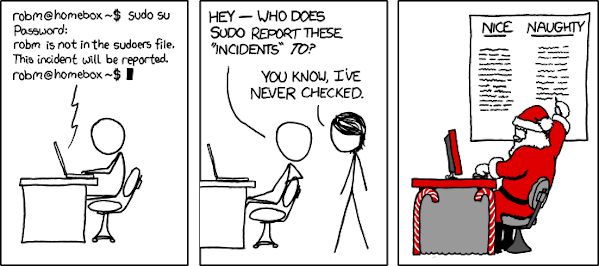
\includegraphics[scale=0.48]{incident.png} \\
IMPORTANT INSTRUCTIONS: \\
\url{https://files.fosswire.com/2007/08/fwunixref.pdf} $\rightarrow$ print this off and tape it up somewhere in your workspace. \\
Better yet, make your own from the slides in this course! 
\end{frame}

\begin{frame}{Credits}
\center
\vspace{8em}
Some of the contents of these slides were liberally borrowed (with permission) from slides from the Winter 2020 offering of 1XA3 (by Curtis D'Alves), and the Winter 2021 offering of 1XC3 (by Dr. Kevin Browne).  
\end{frame}

\end{document}